\chapter[ ]{}
\label{appendix_b}
\section{Stability of Pure Pursuit under time delay}
\label{app:ollero}
The kinematic model shown in Equation \ref{eqn:ppRobotModel}  and first order model for steering dynamics for the vehicle was assumed. 
\begin{equation}
\label{eqn:ppRobotModel}
\begin{pmatrix}
\dot{x'}_w\\ \dot{y'}_w\\ \dot{\theta}
\end{pmatrix}
=
\begin{pmatrix}
-V \sin\theta\\ V\cos\theta\\V\gamma
\end{pmatrix}
\end{equation}
\begin{equation}
\label{eqn:ppSteering}
\frac{d\gamma'}{dt}=-\frac{1}{T}(\gamma'-\gamma_R)
\end{equation}
where, $(x',y',\theta)$ is the posture of robot in coordinate system attached to the robot,  $V$  is the longitudinal velocity,  $\gamma$ is the angular velocity, $T$ time constant of steering dynamics and $\gamma_r$ the control input.  Since the control input is generated by Pure Pursuit it is given by
\begin{eqnarray}
\gamma_r=\frac{1}{r}=\frac{2x}{L^2}
\end{eqnarray} 
where $r$ is defined in Equation \ref{ppControl} and $L$ is the \textit{look ahead distance}. The above Equations \ref{eqn:ppRobotModel} and \ref{eqn:ppSteering}  using the fact that $\dot{y'}_w=0$, because of the non-holonomic constrain of the robot, can be written  in the form of state space  form  as 
\begin{equation}
\begin{pmatrix}
\dot{x}\\\dot{\theta}\\\dot{\gamma}
\end{pmatrix}
=
\begin{pmatrix}
-\sin\theta\\ \gamma \\ -\gamma -\frac{2x}{l^2}
\end{pmatrix}
\end{equation}
where the following scaling of variables were used to render it non-dimensional. 
\begin{equation*}
t=\frac{t'}{T}, \quad x=\frac{x'_w}{VT}, \quad \gamma=VT\gamma',\quad l=\frac{L}{VT}
\end{equation*}
The above system was linearised about the origin and  delay $\tau$ in  input was introduced  to get Equation \ref{eqn:delayPP}
\begin{equation}
\label{eqn:delayPP}
\begin{pmatrix}
\dot{x}\\\dot{\theta}\\\dot{\gamma}
\end{pmatrix}
=J
\begin{pmatrix}
x(t)\\\theta(t)\\\gamma(t)
\end{pmatrix}+
J_\tau 
\begin{pmatrix}
x(t-\tau)\\\theta(t-\tau)\\\gamma(t-\tau)
\end{pmatrix}
\end{equation}
where $J$ is the Jacobian with respect to state and $J_\tau$ is Jacobian with respect to $\tau$. 
Based on location of roots of the Characteristic Quasi-Polynomial $q(s)=det[sI-J-J_\tau~ e^{s\tau} ] $, results for different input delay a limiting  look ahead distance for stable path tracking was presented for a  circular path. His results are represented here for  in Figure \ref{fig:resultsPP}.
  \begin{figure}[h]
  	\centering
	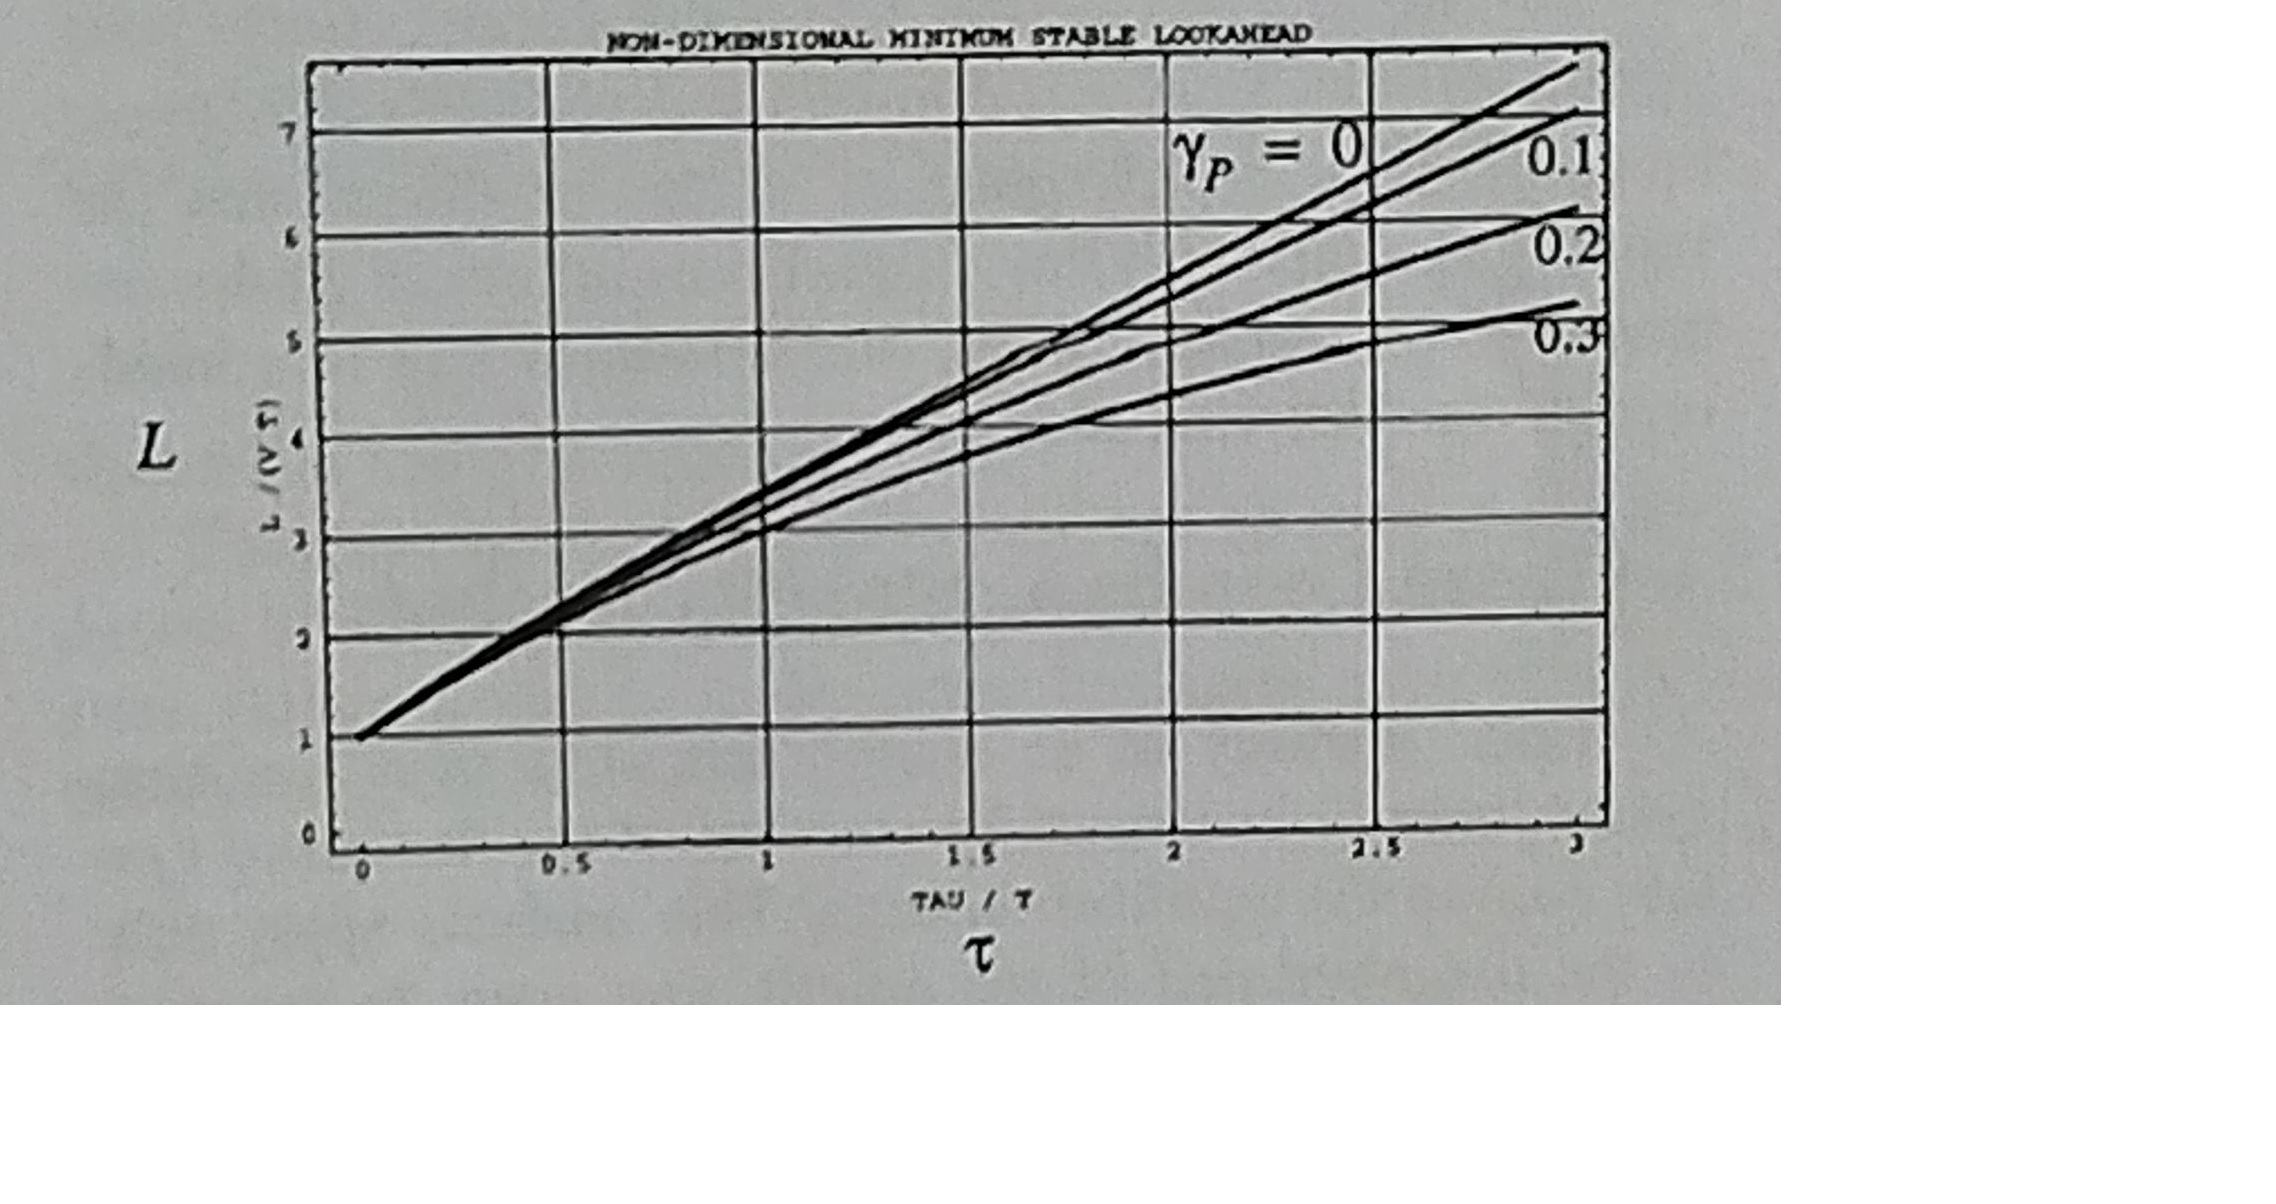
\includegraphics[width=.7\linewidth]{Chapter7/fig/resultsPP}
	\caption{Results obtained by Ollero \cite{ollero1995stability} }
	\label{fig:resultsPP}
\end{figure}